\reportheading{6. Main and branch duct sizing (Task 4)}
\subhead{6.1 Airflow and available cross-section}
Each duct section carries the sum of its downstream peak flows, and its width and depth determine the air velocity through $v=\frac{Q}{WH}$, where W and H are in metres. The design velocity limits are 10 m/s for main ducts and 8 m/s for branch ducts, combined with a width-to-depth ratio of up to 4:1. In addition, a 600 mm depth cap and a 1.0 Pa/m friction target guide duct selection, while the upper friction is limited at 1.23 Pa/m.

A-01 carries the entire 13.0913 m³/s, and thus, at 10 m/s, the minimum duct area is 1.3091 m². With a 600 mm depth, this requires at least 2.182 m of width, and selecting 2200 × 600 mm gives 9.918 m/s and a 3.67:1 width-to-depth ratio. For the branch serving VAV-20, D-44 carries 0.7665 m³/s through a 450 × 300 mm section, giving 5.678 m/s against its 8 m/s limit.

\subhead{6.2 Straight-duct friction}
The drawing provides the equivalent-round Darcy friction gradient at a surface roughness of 0.09 mm. Each section was checked independently in the metric Online Ductulator [5] using the same peak flow and rectangular dimensions, and Appendix D lists both friction results for every section.

\tabletitle{Table 4. Fixed-section check against Online Ductulator [5].}
\begin{reporttable}{L{.16}L{.25}L{.20}L{.19}L{.20}}
\rowcolor{tablegrey} Section & Size (mm) & Online m/s & Online Pa/m & Darcy Pa/m \\\hline
A-01 & 2200 × 600 & 9.9 & 0.877 & 0.9023 \\
D-08 & 1350 × 600 & 9.7 & 0.979 & 0.9995 \\
D-44 & 450 × 300 & 5.7 & 0.980 & 0.9990 \\
\end{reporttable}
The largest displayed online friction gradient is 0.980 Pa/m at D-24 and D-44, while D-08 governs the Darcy check at 0.9995 Pa/m, and both maximum values remain below 1.23 Pa/m. D-44 explains how important the branch schedule is, as it carries only 0.7665 m³/s, but its smaller cross-section gives a higher online friction gradient than the full-flow trunk A-01. However, since these are straight-section pressure gradients, the duct depth and width must still be checked against beams, insulation and crossing services.

{\centering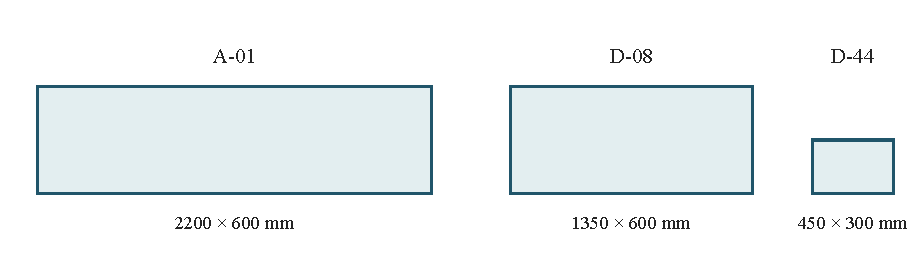
\includegraphics[width=\linewidth]{figures/duct-sections.pdf}\par}
\reportfigure{}{Figure 5. Bare duct cross-sections drawn to a common scale.}
A-01 and D-08 both reach the 600 mm depth cap, and their different widths adjust for the drop in airflow downstream. In contrast, D-44 carries much less air and can use a smaller duct depth. On the common trunk, any loss of usable width at a beam or service crossing reduces the area available at the selected depth. Therefore, the 2200 mm width is essential when coordinating the ceiling as well as when calculating velocity.
